% !TEX TS-program = xepythontex



\documentclass[10pt,envcountsect,spanish]{beamer}


\newif\ifnotas
\notasfalse% Para no mostrar los globos
\notastrue % Para  mostrar los globos

\input ../preambulo.tex


\fvset{frame=leftline, vspace=0pt, fontsize=\small, xleftmargin=.4in, breaklines}


%································ TITULO, AUTOR, ETC
\title{Tipos de Datos Abstractos Sin Orden Lineal}
\subtitle{Tecnología de la Programación}


\author[L. Daniel Hernández]{L. Daniel Hernández $<ldaniel@um.es>$}

\institute[ldaniel@um.es]{Dpto. Ingeniería de la Información  y las Comunicaciones\\ Universidad de Murcia\\\today\\\,\\\hrule} %	 \\ \today\\ \hrule}


\date[ldaniel@um.es]{ 
\vskip 1.25cm
%\vskip -1.25cm
%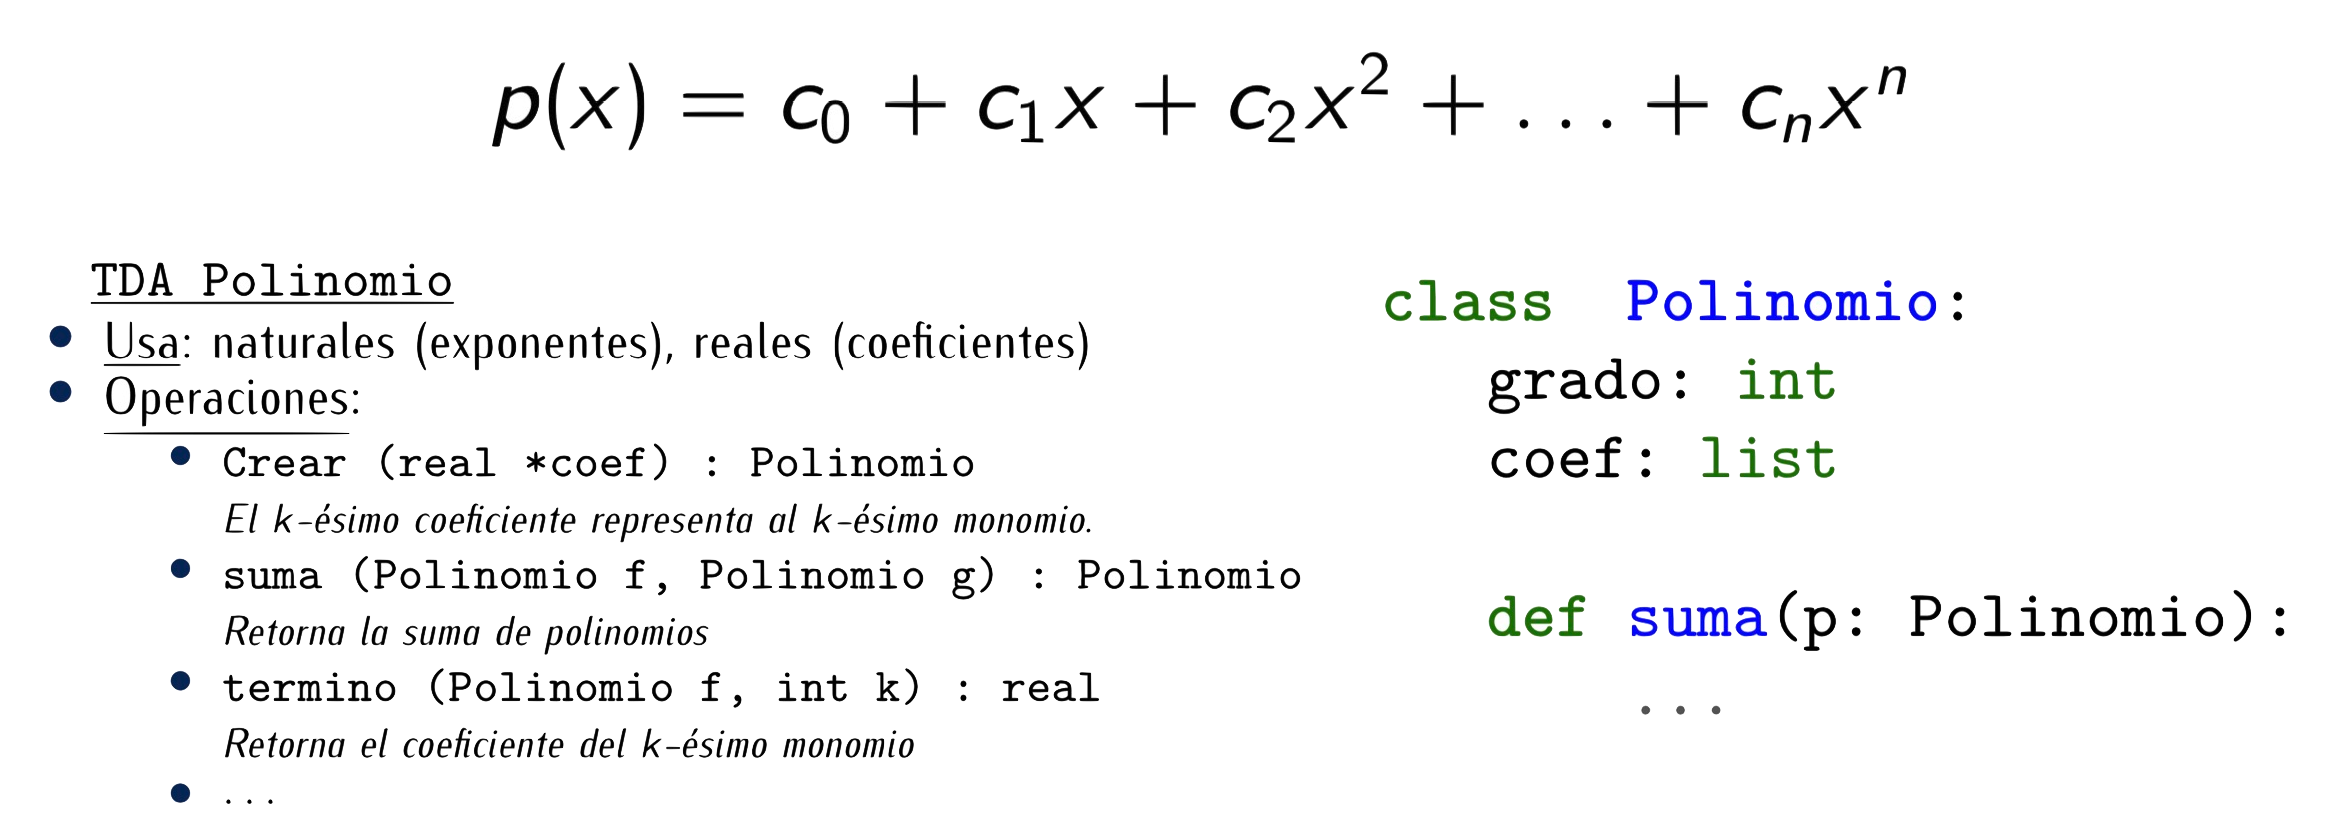
\includegraphics[width=.8\textwidth, height=.18\textheight]{fig/polinomio}
}

\graphicspath{{img/}}



%%%%%%%%%%%%%%%%%%%%%%%%%%%%%%%%%%
%%%%%%%%%%%%%%%%%%%%%%%%%%%%%%%%%%
%%%%%%%%%%%%%%%%%%%%%%%%%%%%%%%%%%
%%%%%%%%%%%%%%%%%%%%%%%%%%%%%%%%%%

%https://es.overleaf.com/learn/how-to/Writing_Markdown_in_LaTeX_Documents
\usepackage[hashEnumerators]{markdown}


%%%%%%%%%%%%%%%%%%%%%%%%%%%%%%%%%%
%%%%%%%%%%%%%%%%%%%%%%%%%%%%%%%%%%
%%%%%%%%%%%%%%%%%%%%%%%%%%%%%%%%%%
%%%%%%%%%%%%%%%%%%%%%%%%%%%%%%%%%%
\begin{document}

%\pgfdeclareimage[height=1cm]{logo}{logo.png}
%\logo{\pgfuseimage{logo}}



%--------------------------------------------------------------------------------
{\usebackgroundtemplate{%
  \includegraphics[width=\paperwidth,height=\paperheight]{../img/fondoUMUCompleto}}
\begin{frame}[b]
	\maketitle

\begin{tikzpicture}[overlay, remember picture]
\node[anchor=south west, %anchor is bottom left corner of the graphic
      xshift=.4\textwidth, %shifting around
      yshift=0.7cm] 
     at (current page.south west) %left bottom corner of the page
     {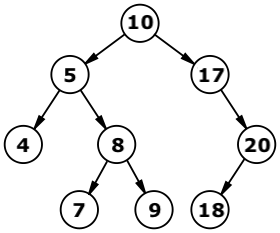
\includegraphics[width=.35\textwidth, height=.3\textheight]{fig/BinarySearchTree}}; 
\end{tikzpicture}
	
\end{frame}			% Transparencia: Título
}



%--------------------------------------------------------------------------------
%%%%%%%%%%%%%%%%%%%%%%%%%%%%%%%%%%
%%%%%%%%%%%%%%%%%%%%%%%%%%%%%%%%%%
\begin{frame}{Índice de Contenidos}\tableofcontents \end{frame}


%%%%%%%%%%%%%%%%%%%%%%%%%%%%%%%%%%%%%
%%%%%%%%%%%%%%%  SECTION   %%%%%%%%%%%%%%%
%%%%%%%%%%%%%%%%%%%%%%%%%%%%%%%%%%%%%
\section{TDAs con Orden Lineal}


%%%%%%%%%%%%%%%%%%%%%%%%%%%%%%%%%%
%%%%%%%%%%%%%%%%%%%%%%%%%%%%%%%%%%
\begin{frame}{Qué son los TDAs sin relación de orden}

\begin{itemize}%\setlength{\itemsep}{0mm}

\item Los TDA con \key{ordenación lineal} son aquellos que contienen a un conjunto de objetos pero donde cada objeto tiene exactamente un predecesor inmediato o un sucesor inmediato. 

\item Los TDA con \key{sin ordenación lineal} son aquellos que contienen a un conjunto de objetos pero donde cada objeto puede tener de 0 a varios sucesores.  

\item Podemos distinguir dos tipos de ordenaciones:

\begin{itemize}
\item Ordenación jerárquica.
\item Ordenación parcial.
\end{itemize}

\end{itemize}
\end{frame}



%%%%%%%%%%%%%%%%%%%%%%%%%%%%%%%%%%
%%%%%%%%%%%%%%%%%%%%%%%%%%%%%%%%%%
\begin{frame}[allowframebreaks]{TDAs con Relación Jerárquica - }

\begin{itemize}
\item Los TDAs con \key{ordenación jerárquica} quedan definidos mediante una relación binaria $a\preceq b$, que será una ordenación no lineal sii hay un solo objeto \textbf{raíz} $r$ (un solo primer elemento) y se cumple:
\begin{itemize}
\item Para todo $a$, $a\preceq a$ (Reflexiva),
\item Para todo $a$, existe $r$ verificando $r\preceq a$ (existe un mínimo en el orden).
\item Si $a\preceq c$ y $b\preceq c$, esto implica que $a\preceq b$ o $b\preceq a$.
\item La relación es antisimétrica:  $a\preceq b$ y $b\preceq a$, esto implica que $a=b$
\item Es transitiva:  $a\preceq b$ y $b\preceq c$, esto implica que $a\preceq c$
\end{itemize}

\item En este orden  pueden existir \key{elementos no comparables}. 


\item Los elementos tienen \key{nombre} en un orden jerárquico:
\begin{itemize}
\item Si $a\preceq b$, $a$ es \textbf{padre} de $b$ y $b$ es \textbf{hijo} de $a$.
\item Cualquier objeto $x$ que cumpla $a\preceq x$ es un \textbf{descendiente} o sucesor de $a$.
\item Cualquier objeto $x$ que cumpla $x\preceq b$ es un \textbf{ascendiente} o ancestro de $b$.
\item El primer elemento de la ordenación recibe el nombre de \textbf{raíz}, y por tanto cumple que solo tiene descendientes y no tiene padre.
\item Los elementos que no tienen hijos se llaman \textbf{hojas}.
\item Los que no son ni hojas ni raíz se llaman \textbf{intermedios}.
\end{itemize}


\framebreak


\item \key{Las operaciones} que se pueden realizar en un orden jerárquico son:
\begin{itemize}
\item \textit{Acceder} directamente al objeto raíz.
\item Dado un objeto \textit{acceder} a su padre y a sus hijos.
\item \textit{determinar} si es la raíz o es una hoja.
\item Dados dos objetos, \textit{encontrar el primer ancestro común}.
\item Dados dos objetos, \textit{encontrar el  recorrido} para llegar de uno a otro.
\item Hacer un \textit{recorrido por todos}  los descendientes de un objeto.
\item \textit{Eliminar} un objeto y todos sus descendientes.
\end{itemize}

\end{itemize}

\end{frame}





%%%%%%%%%%%%%%%%%%%%%%%%%%%%%%%%%%
%%%%%%%%%%%%%%%%%%%%%%%%%%%%%%%%%%
\begin{frame}{TDAs con Relación Parcial}

\begin{itemize}

\item En esta ordenación lo que no puede ocurrir es que dado un objeto, nos lo volvamos a encontrar siguiendo la relación de orden. Es decir, $a\preceq b\preceq \ldots, \preceq a $ no puede darse: es un orden en el que \key{no se permiten ciclos}.


\item Los TDAs con \key{ordenación parcial} quedan definidos mediante una relación binaria $a\preceq b$, que será una ordenación no lineal sii se cumple:
\begin{itemize}
\item Relación reflexiva: Para todo $a$, $a\preceq a$.
\item Relación es antisimétrica:  $a\preceq b$ y $b\preceq a$, esto implica que $a=b$
\item Es transitiva:  $a\preceq b$ y $b\preceq c$, esto implica que $a\preceq c$
\end{itemize}

\item En este orden  pueden existir \key{elementos no comparables}. 


\item Los elementos tienen \key{nombre} en un orden parcial: Reciben los mismos nombres que si tuvieran una ordenación jerárquica (raíz, hijo, intermedio, etc).


\item Algunas \key{operaciones} que se pueden realizar en un orden jerárquico son:

\begin{itemize}
\item \textit{Acceder} a todos los objeto raíces.
\item Dado un objeto \textit{acceder} a sus padres y a sus hijos, \textit{determinar} si es una raíz o es una hoja.
\item Dados dos objetos, \textit{encontrar} el primer ancestro común o el recorrido para llegar de uno a otro.
\item Hacer un \textit{recorrido} por todos todos los objetos
\end{itemize}

\end{itemize}

\end{frame}





%%%%%%%%%%%%%%%%%%%%%%%%%%%%%%%%%%%%%
%%%%%%%%%%%%%%%  SECTION   %%%%%%%%%%%%%%%
%%%%%%%%%%%%%%%%%%%%%%%%%%%%%%%%%%%%%
\section{TDA Árbol}



%%%%%%%%%%%%%%%%%%%%%%%%%%%%%%%%%%%%%
%%%%%%%%%%%%%%%  SECTION   %%%%%%%%%%%%%%%
%%%%%%%%%%%%%%%%%%%%%%%%%%%%%%%%%%%%%
\subsection{Definición del TDA Árbol}

%%%%%%%%%%%%%%%%%%%%%%%%%%%%%%%%%%
%%%%%%%%%%%%%%%%%%%%%%%%%%%%%%%%%%
\begin{frame}{Definición Recursiva del TDA Árbol}

\begin{itemize}%\setlength{\itemsep}{0mm}

\item Un \key{árbol} \label{def:arbol} responde a la siguiente definición recursiva que consta de los siguientes casos:
\begin{itemize}
\item \textbf{Caso base:} El \key{conjunto vacío}  es un árbol. El árbol vacío.
\item \textbf{Caso recursivo:} Un árbol es una colección de datos que está formada por \key{un dato}, $r$, \key{y una lista} de 0 o más árboles, $A_1, A_2, \ldots A_n$.
\end{itemize}

\item  Se deberá  cumplir una ordenación jerárquica donde:
\begin{itemize}
\item Cada dato $r$ será el elemento raíz del árbol que se esté definiendo, y será padre de las raíces de los árboles $A_i$. 
\item Los árboles $A_i$ se llaman subárboles del árbol cuya raíz es $r$.
\end{itemize}



\item Está definición nos da un método de \key{construcción estructural}, empezando por construir el árbol vacío. ¡¡ Hágase !!

\item A los objetos de un árbol se les llama \key{vértices} o \key{nodos}, pero no debe confundir una \key{estructura de datos de tipo nodo} (estructura enlazada de datos). 

\end{itemize}
\end{frame}



%%%%%%%%%%%%%%%%%%%%%%%%%%%%%%%%%%
%%%%%%%%%%%%%%%%%%%%%%%%%%%%%%%%%%
\begin{frame}[allowframebreaks]{Operaciones del TDA Árbol - }

\begin{itemize}

\item Operaciones básicas:
\begin{itemize}
\item \cmn{Tree(): Tree}. Crea un nuevo árbol

\item \cmn{append(value, node=pos): None}. Añade un nuevo nodo al árbol con el valor  \cmn{value}. Si se especifica el segundo parámetro, el nuevo nodo será hijo de  \cmn{pos}.

\item \cmn{value(pos): type\_value}. Retorna el contenido del nodo (posición)  \cmn{pos}.

\item \cmn{replace(pos, value): value}. Cambia el valor del nodo de la posición \cmn{pos} por un nuevo valor (el de entrada) y retorna el antiguo valor.

\item \cmn{remove(pos): None}. Elimina el nodo de la posición \cmn{pos}.

\item \cmn{parent(pos): pos}. Retorna la posición del padre para la posición  \cmn{pos}.
Será  \cmn{None} si la posición de entrada se corresponde con la raíz.

\item \cmn{children(pos): container}. Retorna un contenedor iterable con todos los hijos de  \cmn{pos}.

\item \cmn{positions(): container}. Retorna un contenedor iterable con todos los nodos del árbol.

\item \cmn{elements(): container}. Retorna un contenedor iterable con todos los valores del árbol.

\item \cmn{num\_children(pos): int}. Indica el número de hijos que tiene el nodo \cmn{pos}.

\item \cmn{len(): int}. Retorna el número de elementos que tiene el grafo

\item \cmn{depth(pos): int}. Retorna la profundidad del nodo \cmn{pos}.

\item \cmn{height(pos): int}. Retorna la altura del nodo \cmn{pos}.

\item \cmn{root(): pos}. Retorna la posición del nodo raíz del árbol. 

\item \cmn{isRoot(pos): Bool}. Retorna $True$ si la posición \cmn{pos} es el nodo raíz del árbol. Retorna $False$ en otro caso.

\item \cmn{isInternal(pos): Bool}. Retorna $True$ si la posición \cmn{pos} es el de un nodo interno. Retorna $False$ en otro caso.

\item \cmn{isLeaf(pos): Bool}. Retorna $True$ si  \cmn{pos} es un nodo hoja del árbol. Retorna $False$ en otro caso.

\item \cmn{isEmpty(): Bool}. Indica si el árbol está vacío o no.
\end{itemize}


\item  Se pueden ampliar con una gran cantidad de métodos como, por ejemplo:

\begin{itemize}
	
\item \cmn{borrar(): None}. Borrar los nodos empezando por el nivel más profundo.

\item \cmn{copiar(): Tree}. Copiar un árbol empezando por la raíz.

Copia superficila o profunda (a determinar).

\item \cmn{contar(criterio): int}. Contar el número de elementos que cumplan cierto criterio.

\item \cmn{buscar(valor): bool}.   Buscar un elemento en el árbol.

\item \cmn{comparar(arbol): bool}. Indica si el árbol dado coincide con el actual.

\item \cmn{altura(): int}. Calcula la altura del árbol.

\item \cmn{hojas(): int}. Calcula el número de hojas del árbol.

\end{itemize}

\end{itemize}


\end{frame}






%%%%%%%%%%%%%%%%%%%%%%%%%%%%%%%%%%%%%
%%%%%%%%%%%%%%%  SECTION   %%%%%%%%%%%%%%%
%%%%%%%%%%%%%%%%%%%%%%%%%%%%%%%%%%%%%
\subsection{Implementación del TDA Árbol}

%%%%%%%%%%%%%%%%%%%%%%%%%%%%%%%%%%
%%%%%%%%%%%%%%%%%%%%%%%%%%%%%%%%%%
\begin{frame}[fragile]{Implementación del TDA Árbol}

\begin{itemize}


\item Estructura:

\hfil
\begin{minipage}{.3\textwidth}
\begin{pyverbatim}
struct Arbol
   Nodo raiz
\end{pyverbatim}
\end{minipage}
\begin{minipage}{.65\textwidth}
\begin{pyverbatim}
struct Nodo 
   TDato dato
   Secuencia nodosHijos
\end{pyverbatim}
\end{minipage}\/


\item Un árbol vacío es aquel que cumpla arbol.raiz = None.

\item Notar que al ser un Árbol una composición de nodos se debe aplicar \key{delegación}.

Por ejemplo: dos árboles son iguales si lo son cada uno de sus nodos (el dato y la secuencia de hijos).

\item \fbox{Ejercicio:}
\begin{itemize}
\item ¿Cuál es la función de abstracción? $Abst: \mbox{\textbf{rep}} \longrightarrow {\cal A}$

\item ¿Cuál es el invariante de la representación? $I: \mbox{\textbf{rep}} \longrightarrow \mathbb{B}$

\end{itemize}

\end{itemize}

\end{frame}







%%%%%%%%%%%%%%%%%%%%%%%%%%%%%%%%%%%%%
%%%%%%%%%%%%%%%  SECTION   %%%%%%%%%%%%%%%
%%%%%%%%%%%%%%%%%%%%%%%%%%%%%%%%%%%%%
\section{Árboles Binarios}



%%%%%%%%%%%%%%%%%%%%%%%%%%%%%%%%%%%%%
%%%%%%%%%%%%%%%  SECTION   %%%%%%%%%%%%%%%
%%%%%%%%%%%%%%%%%%%%%%%%%%%%%%%%%%%%%
\subsection{Definición de Árbol Binario}

%%%%%%%%%%%%%%%%%%%%%%%%%%%%%%%%%%
%%%%%%%%%%%%%%%%%%%%%%%%%%%%%%%%%%
\begin{frame}{Definición Recursiva del TDA Árbol}

\begin{itemize}%\setlength{\itemsep}{0mm}

\item De entre los árboles 2-ários distinguimos los árboles binarios. 

\item \key{Definición:}

Un \textbf{árbol binario} es un árbol que \textbf{siempre} tiene dos subárboles que reciben el nombre de hijo (o subárbol) izquierdo e hijo (o subárbol) derecho. En un árbol binario los subárboles pueden ser vacíos.


\item Algunos árboles binarios importantes:
\begin{itemize}
\item 
\key{Árbol de búsqueda binario.} Se utiliza en muchas aplicaciones de búsqueda donde los datos entran/salen constantemente, como los objetos map y set en las bibliotecas de muchos idiomas.

\item 
\key{Partición de espacio binario.} Determina que objetos de un escenario deben renderizarse antes. Se utiliza en casi todos los videojuegos 3D.

\item
\key{Montones.} Se usan para implementar colas de prioridad. Estas colas se usan en sistemas operativos (prioridad de procesos) y en algoritmo de búsqueda de caminos (A* se usa en aplicaciones de AI , incluyendo robótica y videojuegos).

\item
\key{Huffman Coding Tree.}  Se utiliza como algoritmo de compresión, como los utilizados por los formatos de archivo .jpeg y .mp3.
\end{itemize}

\end{itemize}

\end{frame}





%%%%%%%%%%%%%%%%%%%%%%%%%%%%%%%%%%%%%
%%%%%%%%%%%%%%%  SECTION   %%%%%%%%%%%%%%%
%%%%%%%%%%%%%%%%%%%%%%%%%%%%%%%%%%%%%
\subsection{Operaciones basadas en recorridos}



%%%%%%%%%%%%%%%%%%%%%%%%%%%%%%%%%%
%%%%%%%%%%%%%%%%%%%%%%%%%%%%%%%%%%
\begin{frame}[fragile, allowframebreaks]{Recorridos en un Árbol Binario - }

\begin{itemize}
\item
\hfil\begin{minipage}{.9\textwidth}
\begin{pyverbatim}[][frame=single, fontsize=\footnotesize]
def recorrido_anchura (nodo):
    cola = Cola()
    cola.encola(nodo)
    while not cola.isEmpty():
        node = cola.desencola()
        accion(node) # P.e. print(node)
        if  nodo.izquierdo is not None:
            cola.encola(nodo.izquierdo)
        if nodo.derecho is not None:
            cola.encola(nodo.derecho)
\end{pyverbatim}
\end{minipage}

\

\item 
\hfil\begin{minipage}{.9\textwidth}
\begin{pyverbatim}[][frame=single, fontsize=\footnotesize]
def recorrido_profundidad (nodo):
    pila = Pila()
    pila.push(nodo)
    while not pila.isEmpty():
        node = pila.pop()
        accion(node) # P.e. print(node)
        if  nodo.izquierdo is not None:
            pila.push(nodo.izquierdo)
        if nodo.derecho is not None:
            pila.push(nodo.derecho)
\end{pyverbatim}
\end{minipage}

\

\framebreak

\item El \textbf{recorrido en profundidad} sigue alguna de las siguientes  3 estrategias recursivas:

\begin{enumerate}
\item Recorrido prefijo.


\hfil\begin{minipage}{.6\textwidth}
\begin{pyverbatim}[][frame=single, fontsize=\footnotesize]
def recorrido_prefijo(nodo):
    accion(nodo)
    recorrido(nodo.izquierdo)
    recorrido(nodol.derecho)
\end{pyverbatim}
\end{minipage}

\item Recorrido infijo.

\hfil\begin{minipage}{.6\textwidth}
\begin{pyverbatim}[][frame=single, fontsize=\footnotesize]
def recorrido_infijo(nodo):
    recorrido(nodo.izquierdo)
    accion(nodo)
    recorrido(nodol.derecho)
\end{pyverbatim}
\end{minipage}

\item Recorrido postfijo.

\hfil\begin{minipage}{.6\textwidth}
\begin{pyverbatim}[][frame=single, fontsize=\footnotesize]
def recorrido_postfijo(nodo):
    recorrido(nodo.izquierdo)
    recorrido(nodol.derecho)
    accion(nodo)
\end{pyverbatim}
\end{minipage}

\end{enumerate}

\end{itemize}

\end{frame}



%%%%%%%%%%%%%%%%%%%%%%%%%%%%%%%%%%
%%%%%%%%%%%%%%%%%%%%%%%%%%%%%%%%%%
\begin{frame}{Operaciones Basadas en Recorridos}{Consultar la documentación para una descripción más detallada}


\begin{itemize}
\item \key{mostrar(arbol)}: Mostrar los elementos de un árbol como si fuera una expresión aritmética:

\begin{itemize}
\item Caso base: Mostrar los elementos de un árbol vacío es  hacer nada.
\item Caso general: Realizar un recorrido infijo (mostrando los nodos)
\end{itemize}

\item  \key{mostrar(arbol)}:  Mostrar los elementos de un árbol como si fuera una estructura de directorio.

\item  \key{borrar(arbol)}:  Borrar los nodos empezando por el nivel más profundo.


\item   \key{copiar(arbol): arbol}: Copiar un árbol empezando por la raíz.



\item  \key{contar(arbol): int}: Contar el número de elementos que cumplan cierto criterio.



\item \key{buscar(arbol, valor): bool}:  Buscar un elemento en el árbol.

\item \key{comparar(arbol1, arbol2): bool}: Comparar dos árboles.

\item \key{altura(arbol): int}:   Calcular la altura de un árbol.

\item  \key{hojas(arbol): int}: Calcular el número de hojas.

\item Y hay más ....
\end{itemize}
\end{frame}



%%%%%%%%%%%%%%%%%%%%%%%%%%%%%%%%%%%%%
%%%%%%%%%%%%%%%  SECTION   %%%%%%%%%%%%%%%
%%%%%%%%%%%%%%%%%%%%%%%%%%%%%%%%%%%%%
\subsection{Árboles Binarios Destacados}



%%%%%%%%%%%%%%%%%%%%%%%%%%%%%%%%%%
%%%%%%%%%%%%%%%%%%%%%%%%%%%%%%%%%%
\begin{frame}{Árbol Binario de Búsqueda.}


\begin{itemize}
\item \key{Arboles  binarios} de búsqueda cumplen la siguientes\textbf{2 propiedades}:
\begin{itemize}
\item El valor del hijo izquierdo es menor que el valor de la raíz.
\item El valor del hijo derecho es mayor que el valor de la raíz.
\end{itemize}

\item Por \key{recursividad}, se cumplirá que
\begin{itemize}
\item todos los descendiente de la rama izquierda son menores que el valor de la raíz.
\item todos los descendiente de la rama derecha son mayores que el valor de la raíz.
\end{itemize}


\item Ejemplo el de la portada.

\item \key{Operaciones} del TDA Árbol Binario de Búsqueda:


\begin{itemize}
\item \texttt{buscar(arbol, valor): bool}. Algoritmo de búsqueda.

\item  \texttt{añadir(arbol, valor)}. Añadir un elemento en el árbol. Los nuevos elemento se añaden siempre como nodos hojas. 
	
\item   \texttt{minimo(arbol): valor}. Buscar el valor mínimo de un árbol.

\item \texttt{maximo(arbol): valor}. Buscar el valor máximo de un árbol.
	
	
\item  \texttt{borrar(arbol, valor): arbol}: Eliminar el nodo que tiene un valor. El árbol resultante tiene que seguir siendo un árbol binario de búsqueda.

\end{itemize}

\end{itemize}

\end{frame}





%%%%%%%%%%%%%%%%%%%%%%%%%%%%%%%%%%
%%%%%%%%%%%%%%%%%%%%%%%%%%%%%%%%%%
\begin{frame}{Montículos (Heap)}


\begin{itemize}
\item Un heap es un árbol binario donde cada nodo consta de una pareja $(clave, valor)$. Existe una ordenación entre los nodos:
\centerline{$(clave, valor) <  (clave', valor') \Leftrightarrow  clave < clave'$} 
 
\item En muchos casos la clave se obtiene a partir del valor. Por ejemplo, si los valores son numéricos entonces se puede usar como clave dicho valor numérico.

\item Todo heap satisface estas dos propiedades:


\item CONTINUARÁ ....
\end{itemize}

\end{frame}


\end{document}



%%%%%%%%%%%%%%%%%%%%%%%%%%%%%%%%%%%%%
%%%%%%%%%%%%%%%  SECTION   %%%%%%%%%%%%%%%
%%%%%%%%%%%%%%%%%%%%%%%%%%%%%%%%%%%%%
\section{Pilas}

%%%%%%%%%%%%%%%%%%%%%%%%%%%%%%%%%%
%%%%%%%%%%%%%%%%%%%%%%%%%%%%%%%%%%
\begin{frame}{Pilas}

\begin{itemize}
\item Una \key{pila} es una lista con el criterio LIFO.

\item Operaciones
\begin{itemize}
\item \cmn{Stack() : Stack}. Crea una nueva pila, inicialmente vacía.

\item \cmn{peek() : value}. Retorna el valor del tope. También se suele usar la signatura \cm[black]{top() : value}.

Para una pila  $<a_0, a_1, \ldots,>$ retornará el valor $a_0$.

\item \cmn{pop() : value}. Retorna el valor del tope y además borra el primer nodo de la pila.

Para una pila  $<a_0, a_1, a_2, \ldots,>$ retornará el valor $a_0$ y la nueva pila es  $<a_1, a_2, \ldots,>$.


\item \cmn{push(value) : None}. Inserta un nuevo nodo en el tope de la lista. 

Para una pila  $<a_0, a_1, a_2, \ldots,>$ y un valor $value$ la pila se modifica para conseguir la pila $<value, a_0, a_1, a_2, \ldots,>$.


\item \cmn{len() : int}. Retorna el número de elementos de la pila.

\item \cmn{isEmpty() : Bool}. Indica si la pila está vacía o no.

\item \cmn{clear() : None}. Limpia la pila y la deja sin elementos.

\end{itemize}

\item MUY IMPORTANTE: No se puede acceder directamente a ningún elemento central.


\end{itemize}

\end{frame}







%%%%%%%%%%%%%%%%%%%%%%%%%%%%%%%%%%%%%
%%%%%%%%%%%%%%%  SECTION   %%%%%%%%%%%%%%%
%%%%%%%%%%%%%%%%%%%%%%%%%%%%%%%%%%%%%
\section{Colas y Colas de Prioridad}

%%%%%%%%%%%%%%%%%%%%%%%%%%%%%%%%%%
%%%%%%%%%%%%%%%%%%%%%%%%%%%%%%%%%%
\begin{frame}{Colas y Colas de Prioridad}

\begin{itemize}
\item Una \key{cola} es una lista con el criterio FIFO.

\item Operaciones
\begin{itemize}
\item \cmn{Queue() : Queue}. Crea una nueva cola, inicialmente vacía.

\item \cmn{peek() : value}. Retorna el valor del primer elemento de la lista, pero no lo borra.  También es usual esta signatura \cm[black]{front() : value}.

\item \cmn{dequeue() : value}. Retorna el primer elemento de la cola borrandolo de la cola. También es usual esta signatura  \cm[black]{top() : value}.

Para la cola  $<a_0, a_1, \ldots,>$ retornará el valor $a_0$.
Se genera un error si la cola está vacía.

\item \cmn{enqueue(value) : None}.
Añade un nuevo elemento al final de la cola

Para la cola  $<a_0, a_1, \ldots, a_{n-1}>$ 
se modificará a la lista $<a_0, a_1, \ldots, a_{n-1}, value>$ 

\item \cmn{len() : int}. Retorna el número de elementos de la cola.

\item \cmn{isEmpty() : Bool}. Indica si la cola está vacía o no.

\item \cmn{clear() : None}. Limpia la cola y la deja sin elementos.

\end{itemize}

\item Una \key{cola de prioridad} es una cola pero que el encolar a un elemento nuevo lo coloca en la posición que le corresponda en el orden. Las demás operaciones son iguales.


\item MUY IMPORTANTE: No se puede acceder directamente a ningún elemento central.

\end{itemize}

\end{frame}






%%%%%%%%%%%%%%%%%%%%%%%%%%%%%%%%%%%%%
%%%%%%%%%%%%%%%  SECTION   %%%%%%%%%%%%%%%
%%%%%%%%%%%%%%%%%%%%%%%%%%%%%%%%%%%%%
\section{Ordenación usando Pilas y Colas}

%%%%%%%%%%%%%%%%%%%%%%%%%%%%%%%%%%
%%%%%%%%%%%%%%%%%%%%%%%%%%%%%%%%%%
\begin{frame}[fragile]{Ordenación}

\begin{pyverbatim}[][frame=single]
def search(initial, goal_test, successors):
  # Nodo = {estado, nodo_padre}
  
  frontera = [Nodo(initial, None)]  # LISTA de nodos que 
                    # contienen a los estados a expandir
  explorados = {initial} # CONJUNTO de estados analizados
  
  mientras que la frontera no esté vacía:
     nodo_actual = extraer un nodo de frontera (y borrarlo) # PILA, COLA (de prioridad)
     estado_actual = estado del nodo_actual
     si goal_test(estado_actual):
         retornar camino solución para el nodo_actual
     para cada estado de successors(estado_actual):
         si estado está en explorados:
             pasar al siguiente estado
         añadir estado a explorados
         añadir el nodo(estado, nodo_actual) a frontera
  retornar None
\end{pyverbatim}

\end{frame}






\end{document}




%%%%%%%%%%%%%%%%%%%%%%%%%%%%%%%%%%%%%
%%%%%%%%%%%%%%%  SECTION   %%%%%%%%%%%%%%%
%%%%%%%%%%%%%%%%%%%%%%%%%%%%%%%%%%%%%
\section{Set}

%%%%%%%%%%%%%%%%%%%%%%%%%%%%%%%%%%
%%%%%%%%%%%%%%%%%%%%%%%%%%%%%%%%%%
\begin{frame}[allowframebreaks]{Set -}


\begin{itemize}%\setlength{\itemsep}{0mm} \footnotesize
\item Un Bag  donde \textbf{no se permite} la repetición de elementos. 

\item Operaciones:
\begin{itemize}
\item \cmn{Set(): Set}. Crea un nuevo conjunto, \textit{set}, inicialmente vacío.

\item \cmn{len(): int}. Retorna el número de elementos en el conjunto.

Para una lista cualquiera $<a_0, a_1, \ldots, a_{n-1}>$ retornará el valor $n$.

\item \cmn{contains(element): bool}. Indica si el elemento \cmn{element} se encuentra en el conjunto. Retorna \cm{True} si está contenido y \cm{False} si no está contenido.

\item \cmn{add(element): None}. Modifica el conjunto añadiendo  el elemento \cmn{element} al conjunto.

\item \cmn{remove(element): None}. Elimina el elemento \cmn{element} del conjunto. Lanza un error si el elemento no existe.


\item \cmn{iterator(): IteratorSet}: Crea y retorna un iterador para el conjunto.


\item \cmn{isSubsetOf(setB): bool}. Determina si un conjunto es subconjunto del conjunto dado. 

Un conjunto A es subconjunto de B si todos los elementos de A están en B.

\item \cmn{equal(setB): bool}. Determina si el conjunto es igual al conjunto dado. 

Dos conjuntos son iguales si ambos contienen el mismo número de elementos y todos los elementos del conjunto está en el conjunto B. Si ambos están vacíos entonces son iguales.


\item \cmn{union(setB): Set}. Retorna un nuevo conjunto que es la unión del conjunto con el conjunto dado.

La unión del conjunto A  con el conjunto de B es un nuevo conjunto que está formado por todos los elementos de A y todos los elementos de B que no están en A.


\item \cmn{difference(setB): Set}.  Retorna un nuevo conjunto que es la diferencia del conjunto con el conjunto dado.

La diferencia del conjunto A  con el conjunto de B es un nuevo conjunto que está formado por todos los elementos de A que no están en B.


\item \cmn{intersect(): Set}.  Retorna un nuevo conjunto que es la intersección del conjunto con el conjunto dado.

La intersección del conjunto A  con el conjunto de B es un nuevo conjunto que está formado por todos los elementos que están en A y también en B.

\end{itemize}

\item Notar que los 6 primeros operadores del TDA Set son análogos a los operadores del TDA Bag. Los restantes son operaciones bien conocidas de los conjuntos matemáticos.


\end{itemize}

\end{frame}




%%%%%%%%%%%%%%%%%%%%%%%%%%%%%%%%%%%%%
%%%%%%%%%%%%%%%  SECTION   %%%%%%%%%%%%%%%
%%%%%%%%%%%%%%%%%%%%%%%%%%%%%%%%%%%%%
\section{Map}

%%%%%%%%%%%%%%%%%%%%%%%%%%%%%%%%%%
%%%%%%%%%%%%%%%%%%%%%%%%%%%%%%%%%%
\begin{frame}{Map}


\begin{itemize}%\setlength{\itemsep}{0mm} \footnotesize
\item Colección de registros no repetidos donde cada uno consta de una clave y un valor. La clave debe ser comparable y es la que se utiliza para poder acceder al valor.

\item Ejemplos: tener las notas de los estudiantes por su identificador de estudiante, los datos fiscales por algún número de identificación, los datos de un conductor por el número de matricula de su vehículo,  etc ... 


\item Operaciones:

\begin{itemize}
\item \cmn{Map(): Map}. Crea un nuevo map vacío.

\item \cmn{len(): int}. Retorna el número de registros clave/valor que existen en el map..

\item \cmn{contains(key): bool}. Indica si la clave \cmn{key} se encuentra en el contenedor. Retorna \cm{True} si la clave está contenida y \cm{False} si no está contenida.


\item \cmn{remove(key): None}. Elimina el registro que tiene como clave el valor \cmn{key}. Lanza un error si el elemento no existe.


\item \cmn{add(key, value): None}. Modifica el map añadiendo el par \cmn{key/value} al contenedor. Si existiera un registro con la clave \cmn{key} se sustituye el par \cmn{key/value} existente por el nuevo par \cmn{key/value}. Retorna \cm{True} si la clave es nueva y \cm{False} si se realiza una sustitución.


\item \cmn{valueOf(key):  TipoValor}.  Retorna el valor asociado a la clave dada. La clave debe de existir en el Map.

\item \cmn{iterator(): IteratorMap}: Crea y retorna un iterador para el conjunto.
\end{itemize}
\end{itemize}

\end{frame}



%%%%%%%%%%%%%%%%%%%%%%%%%%%%%%%%%%%%%
%%%%%%%%%%%%%%%  SECTION   %%%%%%%%%%%%%%%
%%%%%%%%%%%%%%%%%%%%%%%%%%%%%%%%%%%%%
\section{Implementación}


%%%%%%%%%%%%%%%%%%%%%%%%%%%%%%%%%%
%%%%%%%%%%%%%%%%%%%%%%%%%%%%%%%%%%
\begin{frame}[fragile]{Cómo implementar los TDAs sin orden}

\begin{itemize}

\item \key{Estructuras integradas del lenguaje.}

\begin{itemize}
\item Algunas estructuras conocidas son: \cmn{array},  \cmn{list}, \cmn{tuple} y \cmn{dictionary}, \cmn{namedtuple}, \cmn{chainmap}, etc ...

\item Dependerá del lenguaje particular.


\item Python no tiene arrays.
\end{itemize}



\item \key{Estructuras enlazadas.} 

\begin{itemize}
\item Una estructura enlazada es aquella que se construye utilizando como estructura básica un \key{nodo}: 

\begin{pyverbatim}
struct Nodo
   valor: TDA
   referencia1 Nodo
   referencia2 Nodo
   ...
\end{pyverbatim}

\item Es una estructura construida por el programador.

\item Un nodo  sirve para representar muchos conceptos.

Ejemplo: elementos de un conjunto, los de una lista o los vértices de un árbol o un grafo.  

\item Distintos tipos de nodos nos sirve para implementar el mismo concepto de TDA. 

Ejemplo: un conjunto se puede implementar con un una referencia o con dos referencias.
\end{itemize}

\end{itemize}

\end{frame}


%%%%%%%%%%%%%%%%%%%%%%%%%%%%%%%%%%
%%%%%%%%%%%%%%%%%%%%%%%%%%%%%%%%%%
\section{Estructuras útiles de Python}
%%%%%%%%%%%%%%%%%%%%%%%%%%%%%%%%%%
%%%%%%%%%%%%%%%%%%%%%%%%%%%%%%%%%%


\begin{frame}{Estructuras útiles de Python}
%\small 
\begin{itemize}% \setlength{\itemsep}{0mm}
\item Rangos
\item Listas
\item Tuplas
\item Diccionarios
\end{itemize}
\end{frame}

\end{document}

%%%%%%%%%%%%%%%%%%%%%%%%%%%%%%%%%%
%%%%%%%%%%%%%%%%%%%%%%%%%%%%%%%%%%
\subsection{Abstracción de Datos}
%%%%%%%%%%%%%%%%%%%%%%%%%%%%%%%%%%
%%%%%%%%%%%%%%%%%%%%%%%%%%%%%%%%%%
\begin{frame}{Abstracción de Datos}
\begin{itemize}% \setlength{\itemsep}{0mm}
\item Existen 3 tipos (o niveles) de abstracción.
\item \key{Tipos de datos integrados}  (o fundamentales). Son los que ofrecen los lenguajes de programación.

\cm[magenta]{Ejemplo:} En \cm[red]{Python} se distinguen, entre otros\footnote[frame]{\url{https://docs.python.org/es/3/library/stdtypes.html}}:
\begin{itemize}
\item Los tipos de datos simples: numéricos (enteros, reales y complejos) y booleanos.
\item Los tipos de datos compuestos: cadena de caracteres (str), secuencias (rangos, listas y tuplas), mapas (diccionarios), conjuntos.
\end{itemize}


\item \key{Tipos de datos definidos por el usuario} o programador. Son los que pueden diseñar los programadores agrupando todos de datos fundamentales. 

\begin{itemize}
\item array, record, struct, \cm{class}
\end{itemize}

\item \key{Tipos de datos abstractos (TDA).} Construye modelos (matemáticos) usando agrupación de datos.

\begin{itemize}
\item No es lo mismo una estructura de datos formado por dos valores y operar con ellos que trabajar con vectores numéricos 2D con operaciones matemáticas (donde no importa la estructura).
\end{itemize}

\end{itemize}

\end{frame}




%%%%%%%%%%%%%%%%%%%%%%%%%%%%%%%%%%
%%%%%%%%%%%%%%%%%%%%%%%%%%%%%%%%%%
\section{Tipos de Datos Abstractos}
%%%%%%%%%%%%%%%%%%%%%%%%%%%%%%%%%%
%%%%%%%%%%%%%%%%%%%%%%%%%%%%%%%%%%
\begin{frame}{Tipos de Datos Abstractos}

\begin{itemize}
\item  Los \key{Tipos de Datos Abstractos} (TDA) son \textbf{modelos matemáticos} que constan de

\begin{itemize}
\item un nombre publico para 
\item identificar a un conjunto de datos (valores), junto con
\item un conjunto de operaciones bien definidas sobre los datos (como en una estructura algebraica). 
\end{itemize}

\item Como modelo, le es \key{irrelevante} cómo se almacenan o estructuren los datos y cómo se implementan las operaciones.

\item Para todo TDA hemos de abordar \key{tres tareas}: 

\begin{itemize}
\item \textbf{Especificación:} definición del TDA 
\item \textbf{Representación:} estructura con la que representar el TDA.
\item \textbf{Implementación:} cómo implementar la estructura en un lenguaje de programación.
\end{itemize}

\end{itemize}
\end{frame}




%%%%%%%%%%%%%%%%%%%%%%%%%%%%%%%%%%
%%%%%%%%%%%%%%%%%%%%%%%%%%%%%%%%%%
\subsection{Especificación de TDAs}
%%%%%%%%%%%%%%%%%%%%%%%%%%%%%%%%%%
%%%%%%%%%%%%%%%%%%%%%%%%%%%%%%%%%%
\begin{frame}{Especificación de TDAs}

\begin{itemize}
\item La \key{especificación} de un TDA (Datos+Operaciones) se rige por las normas generales de la \textit{\bf Abstracción por Especificación}

\item La especificación consta de \key{tres partes}: nombre y descripción, la definición de los datos y la definición de los operadores.

\item \key{Nombre y descripción.}
\begin{itemize}
\item Se le dará un nombre que identifica al conjunto de datos y las operaciones.
\item Se indicará qué representan.
\end{itemize}


\item \key{Especificación de los datos.}
\begin{itemize}

	
\item Pueden venir dados por reglas.

\unEjemplo Definiciones recursivas (p.e. una lista).


\item Puede usar notaciones matemáticas conocidas.

\unEjemplo Conjuntos conocidos ($\mathbb{N}$, $\mathbb{R}$, ...), conjuntos $\{s_1,s_2,\ldots\}$, intervalos $[a, b]$, expresiones regulares, ... 

\item Nunca se definirá pensando en estructuras concretas de un lenguaje de programación. 

\end{itemize}


\item \key{Especificación de las Operaciones} (abstractas).

\begin{itemize}
\item Se indicará tanto la sintaxis como la semántica de cada una. 
\item Se emplearan las especificaciones de la abstracción procedimental.
\end{itemize}


\item \textbf{IMPORTANTE.} \key{Un TDA define un valor de tipo $T$:} 

\centerline{\it Todos los entes/valores que respondan al TDA $T$ son de tipo $T$.}

\end{itemize}
\end{frame}




%%%%%%%%%%%%%%%%%%%%%%%%%%%%%%%%%%
%%%%%%%%%%%%%%%%%%%%%%%%%%%%%%%%%%
\begin{frame}{Tipos de Operadores de los TDAs}
\begin{itemize}% \setlength{\itemsep}{0mm}
\item Los operadores de un TDA se pueden dividir por su \key{objetivo}:

	\begin{itemize}
	\item \key{Constructores.} \\ Los que indican cuáles son los datos necesarios para construir un valor de tipo $T$.
	\item \key{Modificadores.} \\ Los que construyen un nuevo valor de tipo $T$ a partir de un valor de tipo $T$ dado.
	\item \key{Consulta}. \\ El conjunto de operaciones que a partir de un valor de tipo $T$ retornan un valor, que no es de tipo $T$.
	\end{itemize}

\item Las operaciones de un TDA se pueden dividir por su \key{importancia}:

	\begin{itemize}
	\item \key{Fundamentales,} también llamadas primitivas. Cumplen  dos condiciones:

	\begin{itemize}
		\item \textbf{No se puede quitar ninguna:} La supresión de una de ellas conlleva que encontramos problemas que no se pueden resolver porque nos faltan operaciones.
		\item Ese conjunto de operaciones \textbf{permite construir cualquier otro tipo de operación} sobre el TDA.
		\item \textbf{Todas deben poder usarse:} todas deben estar visibles.
	\end{itemize}

	\item \key{No fundamentales.}

	\begin{itemize}
		\item \textbf{Apoyan la definición de una operación fundamental,} pero no se puede considerar como tal. No deben de usarse (deben estar ocultas)
		\item Las que \textbf{aumentan el conjunto de operaciones} y se construyen a partir de fundamentales (deberían añadirse las menos posibles)
	\end{itemize}

	\end{itemize}

\end{itemize}
\end{frame}





%%%%%%%%%%%%%%%%%%%%%%%%%%%%%%%%%%
%%%%%%%%%%%%%%%%%%%%%%%%%%%%%%%%%%
\begin{frame}{Un ejemplo de definición de TDA.}

$ $\hskip-0.5cm   \unEjemplo \texttt{\underline{TDA Polinomio}}
\begin{itemize} \setlength{\itemsep}{0mm}
\item { Es una expresión algebraica {\footnotesize $p(x)=c_0+c_1x+c_2x^2+\ldots+c_nx^n$ } compuesta por la \textbf{suma} de dos o más monomios (es un \textbf{coeficiente} y una \textbf{variable} con \textbf{exponente}).
No existen dos monomios con el mismo exponente. Todos los monomios usan la misma variable. El $k$-ésimo monomio es el que tiene una variable con coeficiente $\not=0$.
}

\item \underline{Usa}: {  naturales (exponentes), reales (coeficientes)}

\item \underline{Operaciones}:
	\begin{itemize} 
	\item \texttt{Crear (real *coef) : Polinomio} \\
		\textit{ El $k$-ésimo coeficiente representa al $k$-ésimo monomio.}

	\item \texttt{suma (Polinomio f, Polinomio g) : Polinomio}\\
		\textit{ Retorna la suma de polinomios}

	\item \texttt{termino (Polinomio f, int k) : real}\\
		\textit{ Retorna el coeficiente del $k$-ésimo monomio}
		
	\item $etc \cdots$
	\end{itemize}


\item \textbf{NOTA.} Aquí se muestra una versión simplificada. Hay que seguir la especificación procedimental.
\end{itemize}



\end{frame}




%%%%%%%%%%%%%%%%%%%%%%%%%%%%%%%%%%
%%%%%%%%%%%%%%%%%%%%%%%%%%%%%%%%%%
%--------------------------------------------------------------------------------
\subsection{Representación de TDAs}


%%%%%%%%%%%%%%%%%%%%%%%%%%%%%%%%%%
%%%%%%%%%%%%%%%%%%%%%%%%%%%%%%%%%%
\begin{frame}[fragile]{Representación de TDAs}

\begin{itemize}
\item Se debe de elegir una estructura \textbf{rep} indicando qué datos de un valor de tipo $T$ se almacenan en la estructura \textbf{rep}.

 
\item \key{La función de abstracción.} Una función sobreyectiva $Abst: \mbox{\textbf{rep}} \longrightarrow {\cal A}$ 

\item \key{El invariante de la representación.} Es un predicado
$I: \mbox{\textbf{rep}} \longrightarrow \mathbb{B}$ que es cierto para los objetos de \textbf{rep} que sean legítimos.


\

\item \unEjemplo \texttt{\underline{Representación de Polinomios}}
\begin{itemize}[nosep]
\item	 Para los polinomios {\small $p(x)=c_0+c_1x+c_2x^2+\ldots+c_nx^n$ }se opta por la estructura:

\hfil \begin{minipage}{.24\textwidth}
\scriptsize \tt
\begin{pyverbatim}[][frame=single]
struct rep {
   entero grado
   real[] coef
}
\end{pyverbatim}
\end{minipage}




\item \texttt{grado} es \key{un entero} para representar el grado del polinomio, y 
\item \texttt{coef} es \key{una lista} indexada de reales para representar a los coeficientes \\
\texttt{coef} NO ES UN ARRAY.
\item {\ttfamily  \footnotesize
$Abst($r$)=$r.coef[0]+r.coef[1]$x$+r.coef[2]$x^2$ + $\ldots$  \\
$ $ \hfill $\ldots$ + r.coef[r.grado]$x^{\mbox{\texttt{r.grado}}} $
}

\item {\ttfamily 
$I($r$)$=(r.grado$\not<$0) AND r.grado = len(r.coef)
}
\end{itemize}
%}

\end{itemize}

\end{frame}






%%%%%%%%%%%%%%%%%%%%%%%%%%%%%%%%%%
%%%%%%%%%%%%%%%%%%%%%%%%%%%%%%%%%%
%--------------------------------------------------------------------------------
\subsection{Implementación de TDAs}

%%%%%%%%%%%%%%%%%%%%%%%%%%%%%%%%%%
%%%%%%%%%%%%%%%%%%%%%%%%%%%%%%%%%%
\begin{frame}{Implementación de TDAs}


\begin{itemize}
\item \underline{\cm{lenguaje}}: lenguaje de programación en el que se  implementa el TDA.
\item Lo que \textbf{necesita conocer} el usuario del TDA en ese \underline{\cm{lenguaje}} es:
	 \small
	\begin{itemize}
	\item su \key{nombre}, 
	\item su \key{dominio} (conjuntos de datos con los que trabaja y su tipo), 
	\item su \key{interface} (los nombres de las operaciones asociadas). 
	\end{itemize}
	
	Estos 3 elementos caracterizan a un TDA y se llama \key[red]{parte pública}.
	\normalsize
	
\item Lo que \textbf{no necesita conocer} el usuario del TDA en ese \underline{\cm{lenguaje}} es:
	\small
	\begin{itemize} 
	\item la \textbf{estructura de datos} usada (cómo está codificados los conjuntos de datos)
	\item cómo se han \textbf{implementado} los algoritmos (operadores)
	\end{itemize}
	
	Estos elementos reciben el nombre de \key[red]{parte privada}.
	\normalsize
	
\item Cuando se programe el TDA se deberá de tener en cuenta estas dos partes.

\item Se deberá de implementar considerando:

	\small
	\begin{itemize} 
	\item \key{Encapsulamiento,} agrupando en un objeto atributos (variables) y métodos (operaciones).
	\item \key{Ocultación} de información, pues establecer qué atributos y métodos pueden permanecer ocultas (o visibles).
	\end{itemize}
	\normalsize
	
	

	
\item La POO aparece de forma natural para resolver esta situación.


\item \small \key[red]{Nuestro Objetivo:} 

\centerline{\bf \underline{Usar} la POO para \underline{implementar} TDAs (que son modelos matemáticos) \underline{en} \cm[red]{Python}.}

\end{itemize}

\end{frame}


\end{document}


